\documentclass[10pt,twocolumn,letterpaper]{article}

\usepackage[UTF8]{ctex}
\usepackage{cvpr}
\input{preamble}
\usepackage[pagebackref,breaklinks,colorlinks,allcolors=blue]{hyperref}
\usepackage{multirow}
\usepackage{array}

\title{基于双边滤波与引导滤波的低光照图像增强实验报告}

\author{作者信息待填写\\
{\tt\small 学号待填写}}

\begin{document}
\maketitle

\begin{abstract}
本文围绕低光照图像增强任务，基于 Retinex 思想实现了一个最小可运行的增强流程，并重点比较了双边滤波与引导滤波两种边缘保持平滑方法。具体而言，先利用 RGB 三通道最大值估计初始照明图，再分别采用双边滤波和自引导滤波对照明图进行平滑，最后通过照明补偿公式恢复增强图像。实验数据来自题目提供的 10 组低光照/GT 配对样本，定量评价指标包括 PSNR、SSIM、MAE、MSE 和 LPIPS。结果表明，在默认参数下，引导滤波在五项平均指标上整体优于双边滤波。进一步的参数敏感性实验显示，双边滤波对邻域直径 $d$ 最敏感，对值域参数 $\sigma_{color}$ 次之，而空间域参数 $\sigma_{space}$ 的影响相对有限；引导滤波则对窗口半径 $r$ 和正则参数 $\epsilon$ 均较为敏感，其中较大的窗口半径有利于得到更稳定的照明估计，而 $\epsilon$ 体现出保边与过平滑之间的折中；增强参数方面，$T_{\min}$ 与 $\gamma$ 共同决定暗区补偿强度，其中过小的 $T_{\min}$ 容易放大噪声，过大的 $T_{\min}$ 又会抑制亮度恢复，而 $\gamma$ 过小会导致增强不足，过大则会引入明显的过增强。本文实验说明，边缘保持平滑是低光照增强中的关键步骤，而合适的平滑尺度与增强强度决定了最终结果的稳定性与视觉效果。
\end{abstract}

\section{研究现状及主要研究方法}
低光照图像通常存在亮度不足、暗区细节难以辨识、噪声显著以及色彩失真等问题。传统方法中，Retinex 理论认为图像可以表示为反射分量与照明分量的乘积，即
\begin{equation}
I(x)=R(x)\cdot T(x),
\end{equation}
其中 $I(x)$ 为观测图像，$R(x)$ 对应反射信息，$T(x)$ 对应照明信息。低光照增强的基本思想是在估计照明分量后对其进行补偿，从而恢复更合理的反射结果 \cite{land1971retinex}。

从研究路线看，低光照增强大致可以分为三类。第一类是基于图像先验的传统方法，例如直方图均衡、Gamma 校正、Retinex 系列方法以及基于照明图估计的方法。LIME 通过直接估计照明图并施加结构先验，证明了照明建模对增强质量的重要性 \cite{guo2016lime}。第二类是基于边缘保持滤波的增强方法，这类方法通常先从输入图像中估计粗略照明图，再通过双边滤波或引导滤波抑制纹理和噪声，兼顾平滑性与边缘保持 \cite{tomasi1998bilateral,he2010guided,he2013guided}。第三类是深度学习方法，包括 Retinex-Net、KinD、Zero-DCE 等代表性工作，它们能够在大规模训练数据上学习更复杂的亮度映射或分解关系，但通常依赖训练数据、计算资源和更复杂的模型设计 \cite{wei2018retinexnet,zhang2019kind,guo2020zerodce}。

近年来的综述研究指出，传统方法在可解释性、实现成本和小样本场景中仍具有优势，而学习型方法在视觉质量和泛化能力上表现更强 \cite{guo2023survey}。对本次课程作业而言，基于双边滤波与引导滤波的 Retinex 型方法具有结构清晰、参数可解释、便于展示中间结果和分析实验现象等优点，因此适合作为实验报告的主体方案。

\section{本文研究方法}
\subsection{初始照明图估计}
设输入 RGB 低光照图像为 $I$，首先将其归一化到 $[0,1]$，再按照题目要求采用三通道最大值估计初始照明图：
\begin{equation}
T_0(x)=\max\{I_R(x),I_G(x),I_B(x)\}.
\end{equation}
该估计方式实现简单，能够快速反映局部亮度水平，但直接得到的 $T_0$ 往往混入纹理细节、边缘和噪声，因此不能直接作为最终照明图使用。

\subsection{照明图平滑}
为了得到更符合真实照明分布的结果，本文分别采用双边滤波和引导滤波对 $T_0$ 进行边缘保持平滑。

\paragraph{双边滤波}
双边滤波在邻域加权平均时同时考虑空间距离和像素值相似性，其形式为
\begin{equation}
T_b(x)=\frac{1}{W_x}\sum_{y\in\Omega(x)}G_s(\|x-y\|)G_r(|T_0(x)-T_0(y)|)T_0(y),
\end{equation}
其中 $G_s(\cdot)$ 和 $G_r(\cdot)$ 分别对应空间域权重和值域权重，$W_x$ 为归一化因子 \cite{tomasi1998bilateral}。本文实现中使用 OpenCV 的双边滤波接口，重点调节邻域直径 $d$、值域参数 $\sigma_{color}$ 和空间域参数 $\sigma_{space}$。

\paragraph{引导滤波}
引导滤波假设在局部窗口 $\omega_k$ 内，输出 $q$ 与引导图像 $G$ 满足线性关系
\begin{equation}
q_i=a_k G_i+b_k,\quad i\in \omega_k.
\end{equation}
在最小二乘与正则化约束下，可求得局部系数
\begin{equation}
a_k=\frac{\mathrm{cov}_{\omega_k}(G,p)}{\mathrm{var}_{\omega_k}(G)+\epsilon},\quad
b_k=\bar{p}_k-a_k\mu_k,
\end{equation}
其中 $p$ 为待滤波图像，$\epsilon$ 为正则项 \cite{he2010guided,he2013guided}。本文采用自引导方案，即 $G=T_0,p=T_0$，并以窗口半径 $r$ 与正则参数 $\epsilon$ 控制平滑尺度。

\subsection{照明补偿与增强恢复}
在得到平滑后的照明图 $T$ 后，对输入图像进行照明补偿，增强公式写为
\begin{equation}
J_c(x)=\frac{I_c(x)}{\max(T(x),T_{\min})^\gamma},
\end{equation}
其中 $J_c(x)$ 表示输出图像在通道 $c$ 上的像素值，$T_{\min}$ 用于避免极暗区域分母过小导致数值不稳定，$\gamma$ 用于调节增强强度。增强后再将结果裁剪到 $[0,1]$，以便保存图像和计算指标。

\subsection{算法流程}
本文方法可以概括为以下步骤：
\begin{enumerate}
    \item 读取低光照图像并归一化；
    \item 通过 RGB 三通道最大值估计初始照明图 $T_0$；
    \item 对 $T_0$ 分别采用双边滤波或自引导滤波进行平滑；
    \item 利用平滑照明图和增强公式恢复增强结果；
    \item 将增强结果与 Ground Truth 进行对比，计算 PSNR、SSIM、MAE、MSE 和 LPIPS \cite{wang2004ssim,zhang2018lpips}。
\end{enumerate}

\begin{figure}[t]
    \centering
    \subcaptionbox{初始照明图 $T_0$}{
        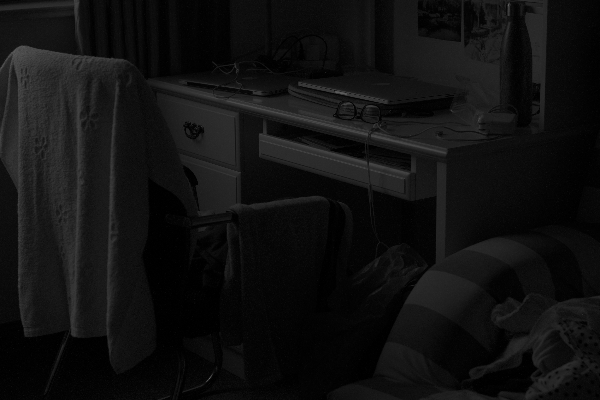
\includegraphics[width=0.31\linewidth]{../assets/figures/t0_default_00017.png}
    }
    \hfill
    \subcaptionbox{双边滤波平滑结果}{
        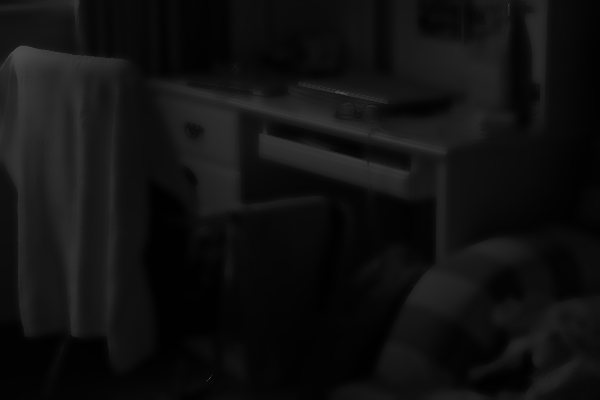
\includegraphics[width=0.31\linewidth]{../assets/figures/smooth_bilateral_default_00017.png}
    }
    \hfill
    \subcaptionbox{引导滤波平滑结果}{
        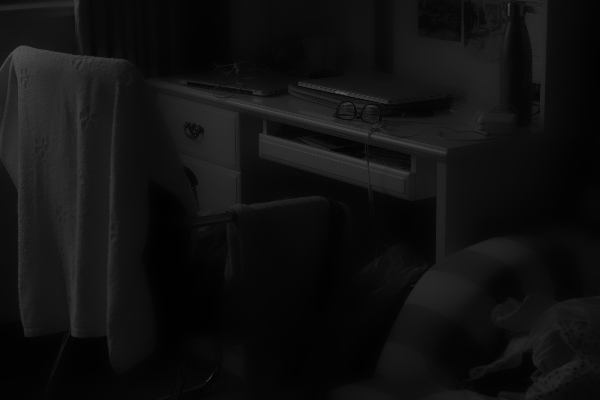
\includegraphics[width=0.31\linewidth]{../assets/figures/smooth_guided_default_00017.png}
    }
    \caption{样本 \texttt{00017.png} 的中间结果示意。双边滤波得到的照明图更平滑，但边缘附近略有扩散；引导滤波保留了更多结构边界。}
    \label{fig:intermediate}
\end{figure}

\section{实验结果}
\subsection{实验设置}
实验数据采用题目提供的 \texttt{samples/Train/Input} 与 \texttt{samples/Train/GT}，共 10 对配对图像。默认参数设置如下：双边滤波为 $d=15,\sigma_{color}=0.1,\sigma_{space}=15$；引导滤波为 $r=8,\epsilon=10^{-3}$；增强参数为 $T_{\min}=0.1,\gamma=0.8$。其中，PSNR、SSIM 越大越好，MAE、MSE、LPIPS 越小越好。

\subsection{默认参数下的方法对比}
表 \ref{tab:main} 给出了默认参数下双边滤波与引导滤波的平均结果。可以看到，引导滤波在五项指标上整体优于双边滤波，其中 PSNR 提升约 $0.15$ dB，SSIM 提升 $0.0176$，LPIPS 降低 $0.0058$。这说明在当前任务中，引导滤波得到的照明图更有利于保留结构边缘并抑制不必要的亮度扩散。

\begin{table}[t]
    \centering
    \caption{默认参数下两种方法的平均指标对比}
    \label{tab:main}
    \begin{tabular}{lccccc}
        \toprule
        方法 & PSNR$\uparrow$ & SSIM$\uparrow$ & MAE$\downarrow$ & MSE$\downarrow$ & LPIPS$\downarrow$ \\
        \midrule
        双边滤波 & 18.3094 & 0.6109 & 0.1135 & 0.0196 & 0.2544 \\
        引导滤波 & \textbf{18.4591} & \textbf{0.6285} & \textbf{0.1122} & \textbf{0.0193} & \textbf{0.2486} \\
        \bottomrule
    \end{tabular}
\end{table}

\begin{figure}[t]
    \centering
    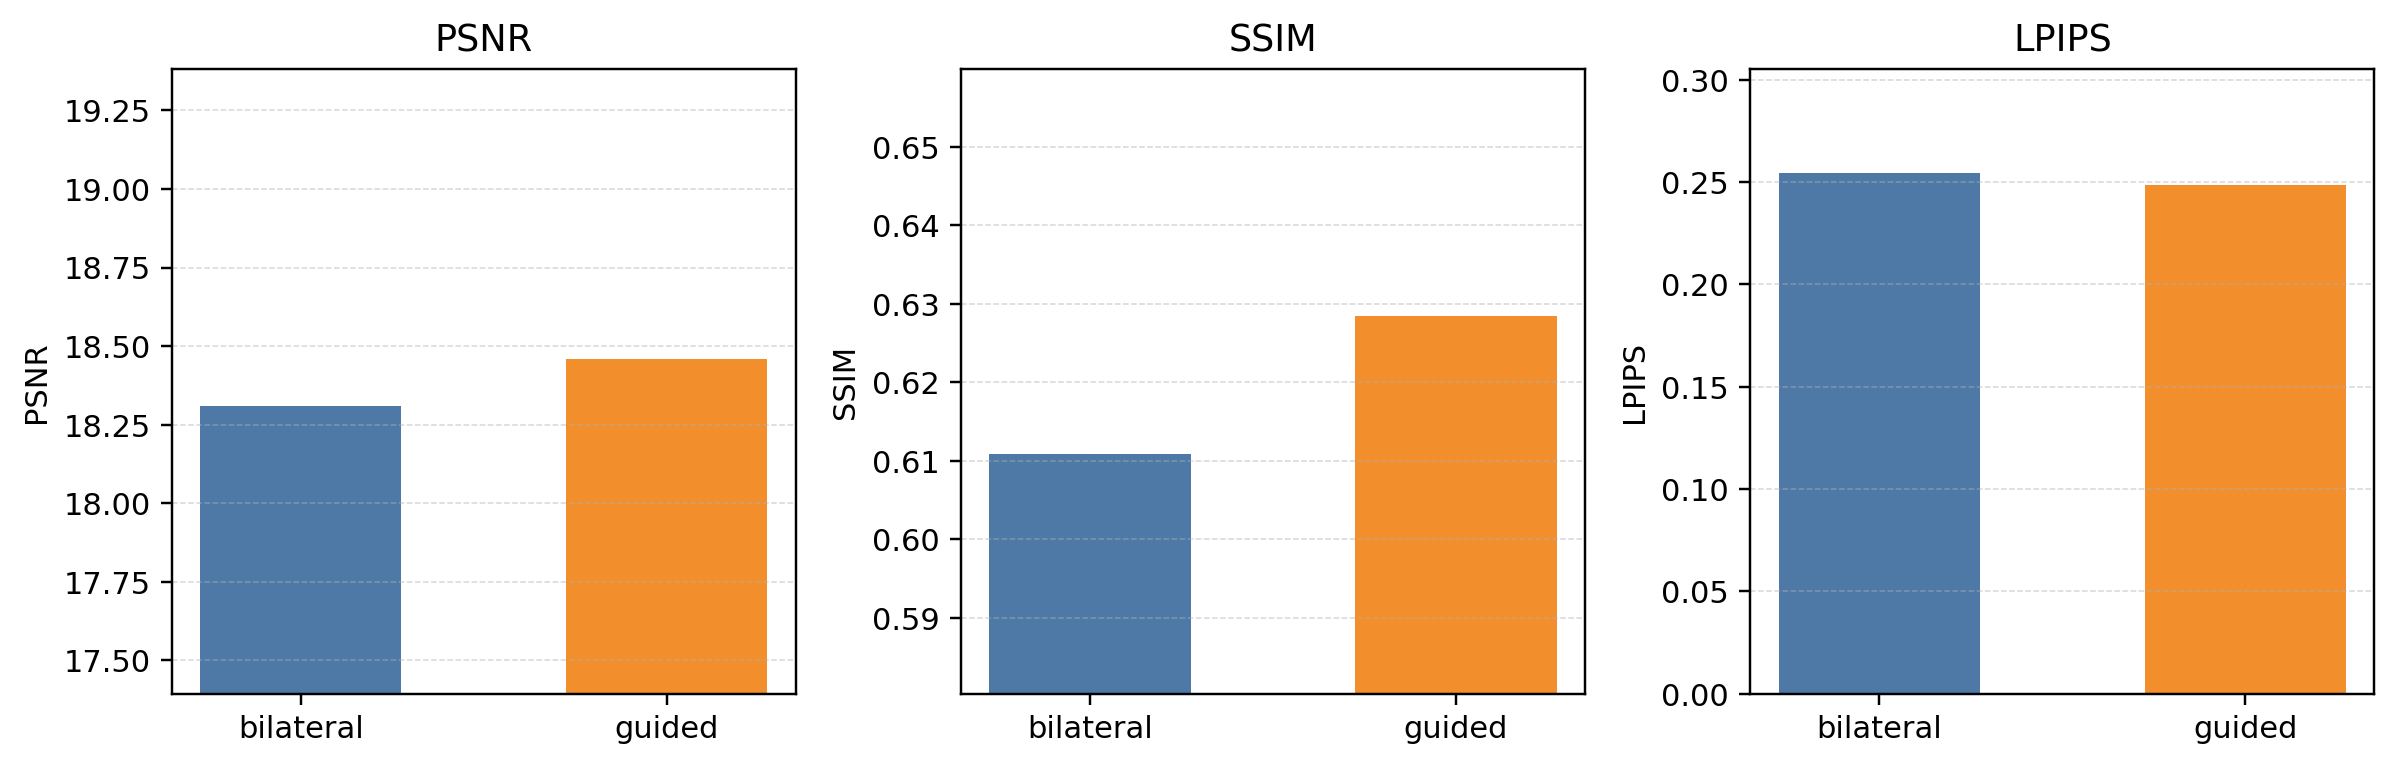
\includegraphics[width=\linewidth]{../assets/figures/main_method_comparison.png}
    \caption{默认参数下双边滤波与引导滤波的平均指标对比图。}
    \label{fig:main_bar}
\end{figure}

进一步查看逐图像结果可知，引导滤波在 10 张样本上均取得更高的 PSNR 与 SSIM；在 LPIPS 上，引导滤波在 8 张样本上优于双边滤波，仅在 \texttt{00001.png} 和 \texttt{00051.png} 上略逊于双边滤波。这表明两种方法在大多数场景下趋势一致，但感知指标与像素级指标并不总是完全同步。

\subsection{定性结果分析}
图 \ref{fig:qual_hard} 展示了较困难样本 \texttt{00017.png} 的结果。该样本原图照明极弱，桌面下方和窗帘区域均存在大面积暗区。两种方法都能显著提升可见性，但增强后仍可观察到明显噪声，且与 GT 相比存在亮度偏差，因此其 PSNR 仅约为 11.9 dB。结合图 \ref{fig:intermediate} 可见，双边滤波后的照明图更加平滑，导致增强结果整体略显“泛灰”；引导滤波保留了更多局部结构，因而 SSIM 略高。

\begin{figure}[t]
    \centering
    \subcaptionbox{双边滤波结果}{
        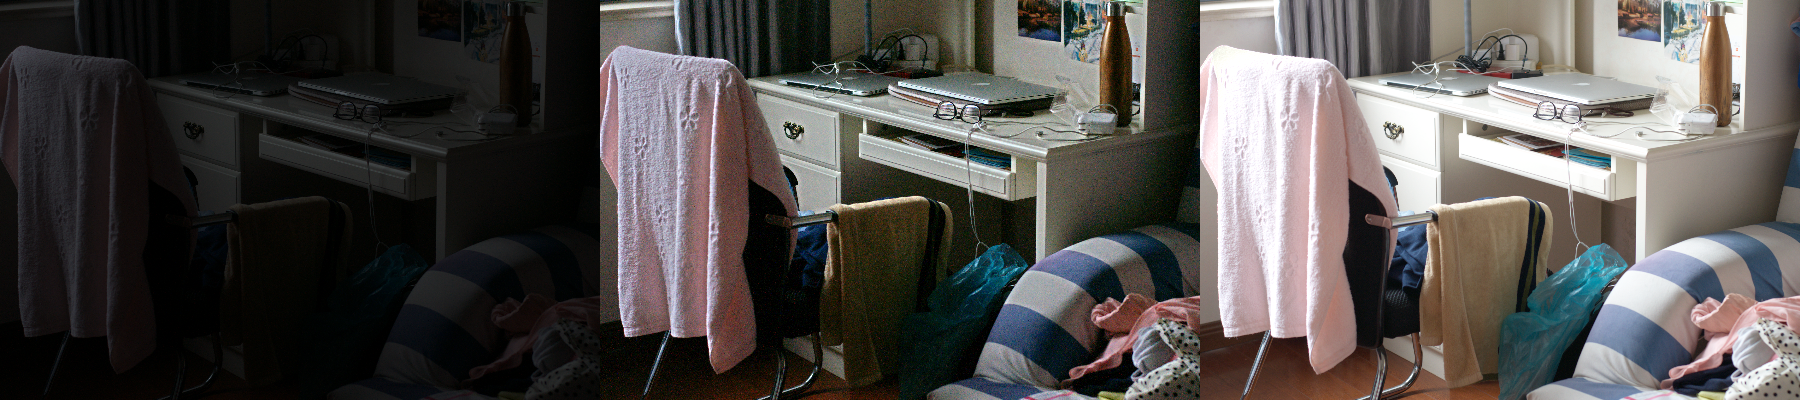
\includegraphics[width=\linewidth]{../assets/figures/comparison_bilateral_default_00017.png}
    }
    \\
    \subcaptionbox{引导滤波结果}{
        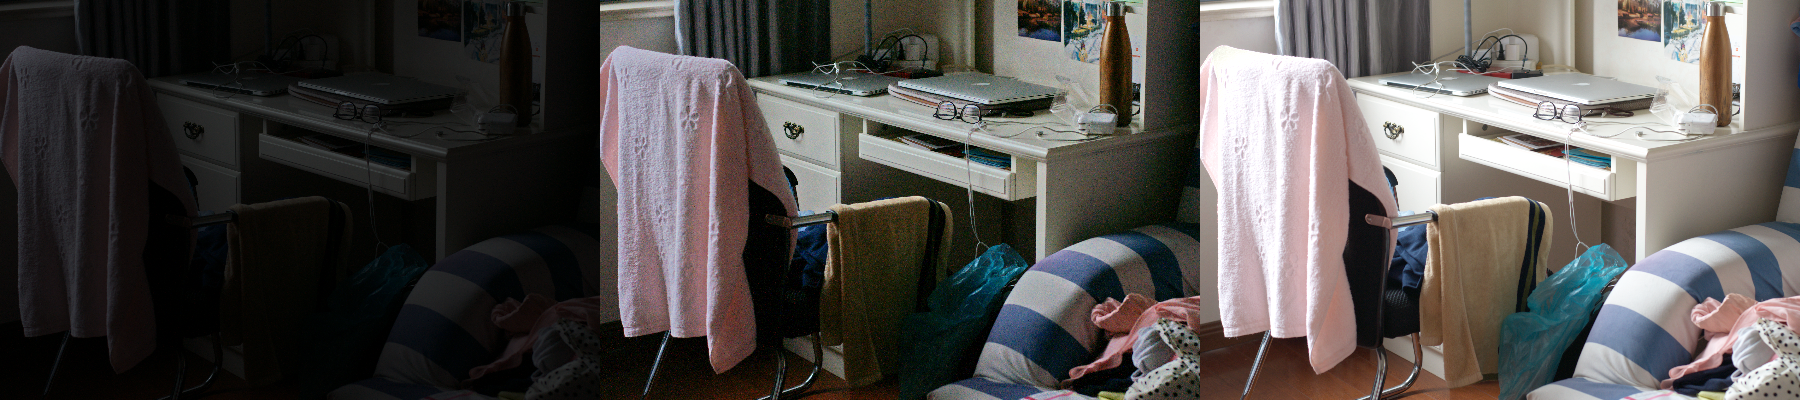
\includegraphics[width=\linewidth]{../assets/figures/comparison_guided_default_00017.png}
    }
    \caption{困难样本 \texttt{00017.png} 的定性结果。每行从左到右分别为输入图像、增强结果和 Ground Truth。}
    \label{fig:qual_hard}
\end{figure}

图 \ref{fig:qual_good} 展示了两个较稳定样本的结果。对 \texttt{00051.png} 而言，引导滤波在植物叶片和椅背边缘处保留了更清晰的结构；对 \texttt{00091.png} 而言，引导滤波能够更好地恢复炉灶边界和锅体轮廓，同时控制墙面区域的亮度泄漏。两者共同说明，引导滤波在结构清晰的场景下更容易获得与 GT 接近的亮度分布。

\begin{figure}[t]
    \centering
    \subcaptionbox{\texttt{00051.png}}{
        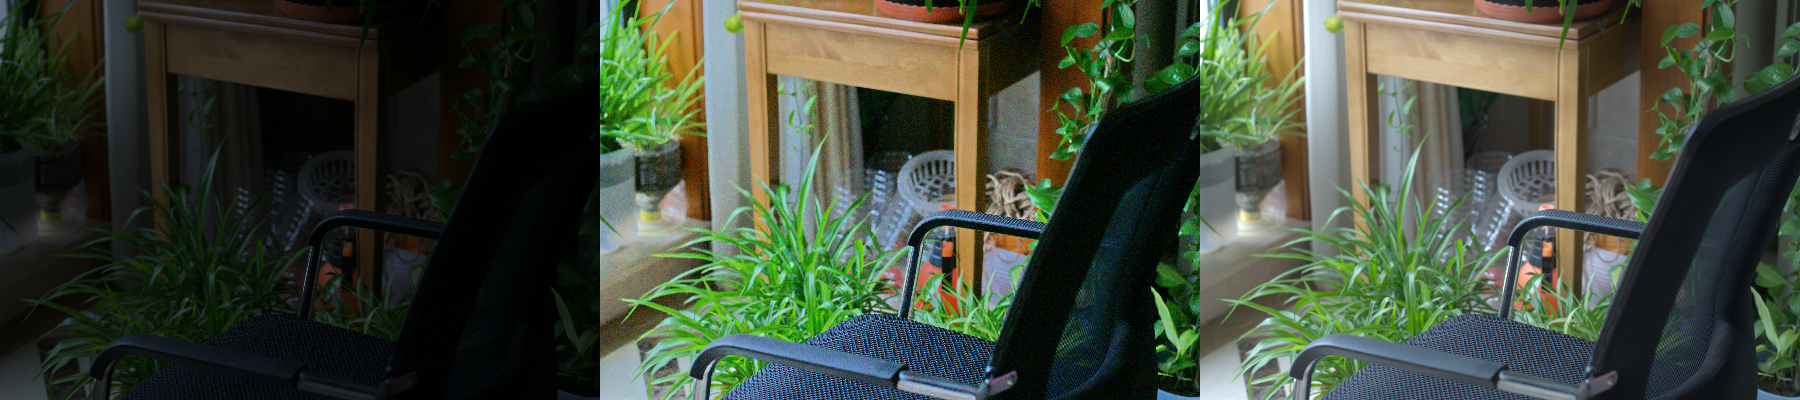
\includegraphics[width=\linewidth]{../assets/figures/comparison_guided_default_00051.png}
    }
    \\
    \subcaptionbox{\texttt{00091.png}}{
        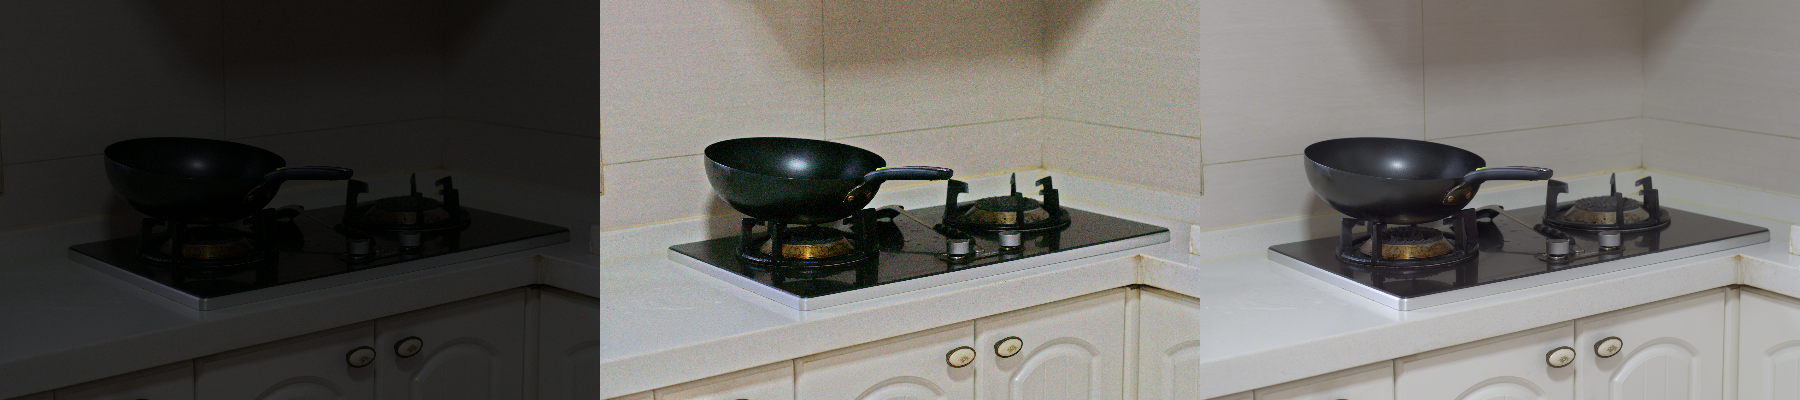
\includegraphics[width=\linewidth]{../assets/figures/comparison_guided_default_00091.png}
    }
    \caption{两个代表性样本的引导滤波增强结果。每行从左到右分别为输入图像、增强结果和 Ground Truth。}
    \label{fig:qual_good}
\end{figure}

\subsection{参数敏感性分析}
为分析中间设计对结果的影响，本文进一步对双边滤波的三个关键参数 $d$、$\sigma_{color}$ 和 $\sigma_{space}$ 进行了更宽范围的控制变量实验；同时扩展了引导滤波的窗口半径 $r$、正则参数 $\epsilon$ 以及增强参数 $T_{\min}$、$\gamma$ 的实验范围。各组实验均固定其余参数为默认值，仅改变单个参数。

\paragraph{双边滤波邻域直径 $d$}
表 \ref{tab:bilateral_diameter} 与图 \ref{fig:bilateral_diameter_curve} 给出了 $d=3,5,9,15,25,35$ 时的结果。随着邻域直径增大，PSNR、SSIM 持续上升，LPIPS 整体下降，其中 $d=35$ 时达到最优。这说明在当前数据集上，较大的邻域窗口有助于对照明图进行更充分的局部平均，使增强结果在整体亮度分布上更接近 GT；但从中间照明图可见，过大的 $d$ 会扩大平滑尺度，弱化局部照明边界。

\begin{table}[t]
    \centering
    \caption{双边滤波邻域直径 $d$ 的影响}
    \label{tab:bilateral_diameter}
    \begin{tabular}{cccc}
        \toprule
        $d$ & PSNR$\uparrow$ & SSIM$\uparrow$ & LPIPS$\downarrow$ \\
        \midrule
        3  & 18.2614 & 0.6104 & 0.2622 \\
        5  & 18.2701 & 0.6106 & 0.2767 \\
        9  & 18.2841 & 0.6108 & 0.2618 \\
        15 & 18.3094 & 0.6109 & 0.2544 \\
        25 & 18.3460 & 0.6130 & 0.2516 \\
        35 & \textbf{18.3785} & \textbf{0.6153} & \textbf{0.2508} \\
        \bottomrule
    \end{tabular}
\end{table}

\begin{figure}[t]
    \centering
    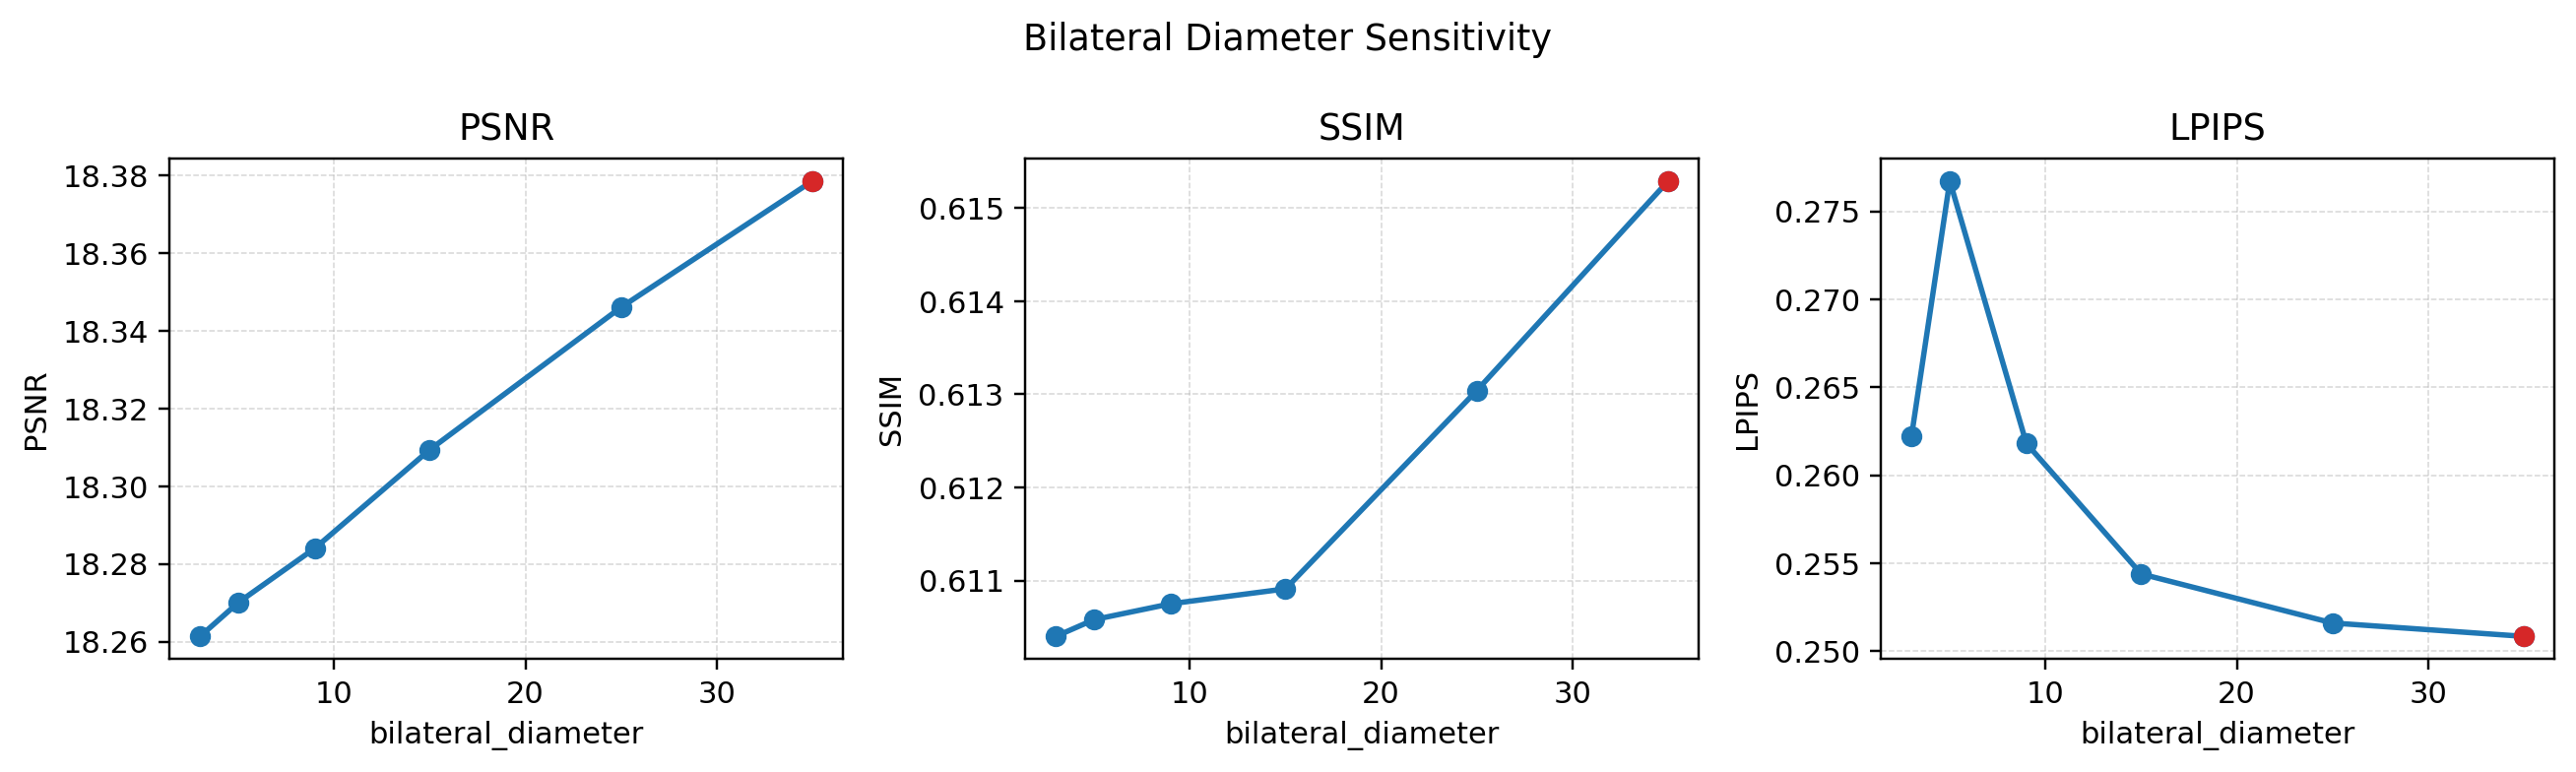
\includegraphics[width=\linewidth]{../assets/figures/bilateral_diameter_curve.png}
    \caption{双边滤波邻域直径变化对平均指标的影响。}
    \label{fig:bilateral_diameter_curve}
\end{figure}

\paragraph{双边滤波值域参数 $\sigma_{color}$}
表 \ref{tab:bilateral_sigma_color} 与图 \ref{fig:bilateral_sigma_color_curve} 展示了 $\sigma_{color}=0.01,0.03,0.05,0.10,0.20,0.40$ 时的实验结果。随着 $\sigma_{color}$ 增大，SSIM 近似单调下降，而 PSNR 呈现先升后降的趋势，在 $\sigma_{color}=0.05$ 附近取得最高值；LPIPS 在 $\sigma_{color}=0.20$ 时最优。该现象说明较小的 $\sigma_{color}$ 更强调值域相似性，对跨边缘混合的抑制更强，因此结构指标更高；当 $\sigma_{color}$ 过大时，边缘约束减弱，照明图容易被过度平滑，细节结构损失更明显。

\begin{table}[t]
    \centering
    \caption{双边滤波值域参数 $\sigma_{color}$ 的影响}
    \label{tab:bilateral_sigma_color}
    \begin{tabular}{cccc}
        \toprule
        $\sigma_{color}$ & PSNR$\uparrow$ & SSIM$\uparrow$ & LPIPS$\downarrow$ \\
        \midrule
        0.01 & 18.2763 & \textbf{0.6257} & 0.2641 \\
        0.03 & 18.3058 & 0.6214 & 0.2627 \\
        0.05 & \textbf{18.3311} & 0.6181 & 0.2578 \\
        0.10 & 18.3094 & 0.6109 & 0.2544 \\
        0.20 & 18.2777 & 0.6057 & \textbf{0.2542} \\
        0.40 & 18.2550 & 0.6035 & 0.2546 \\
        \bottomrule
    \end{tabular}
\end{table}

\begin{figure}[t]
    \centering
    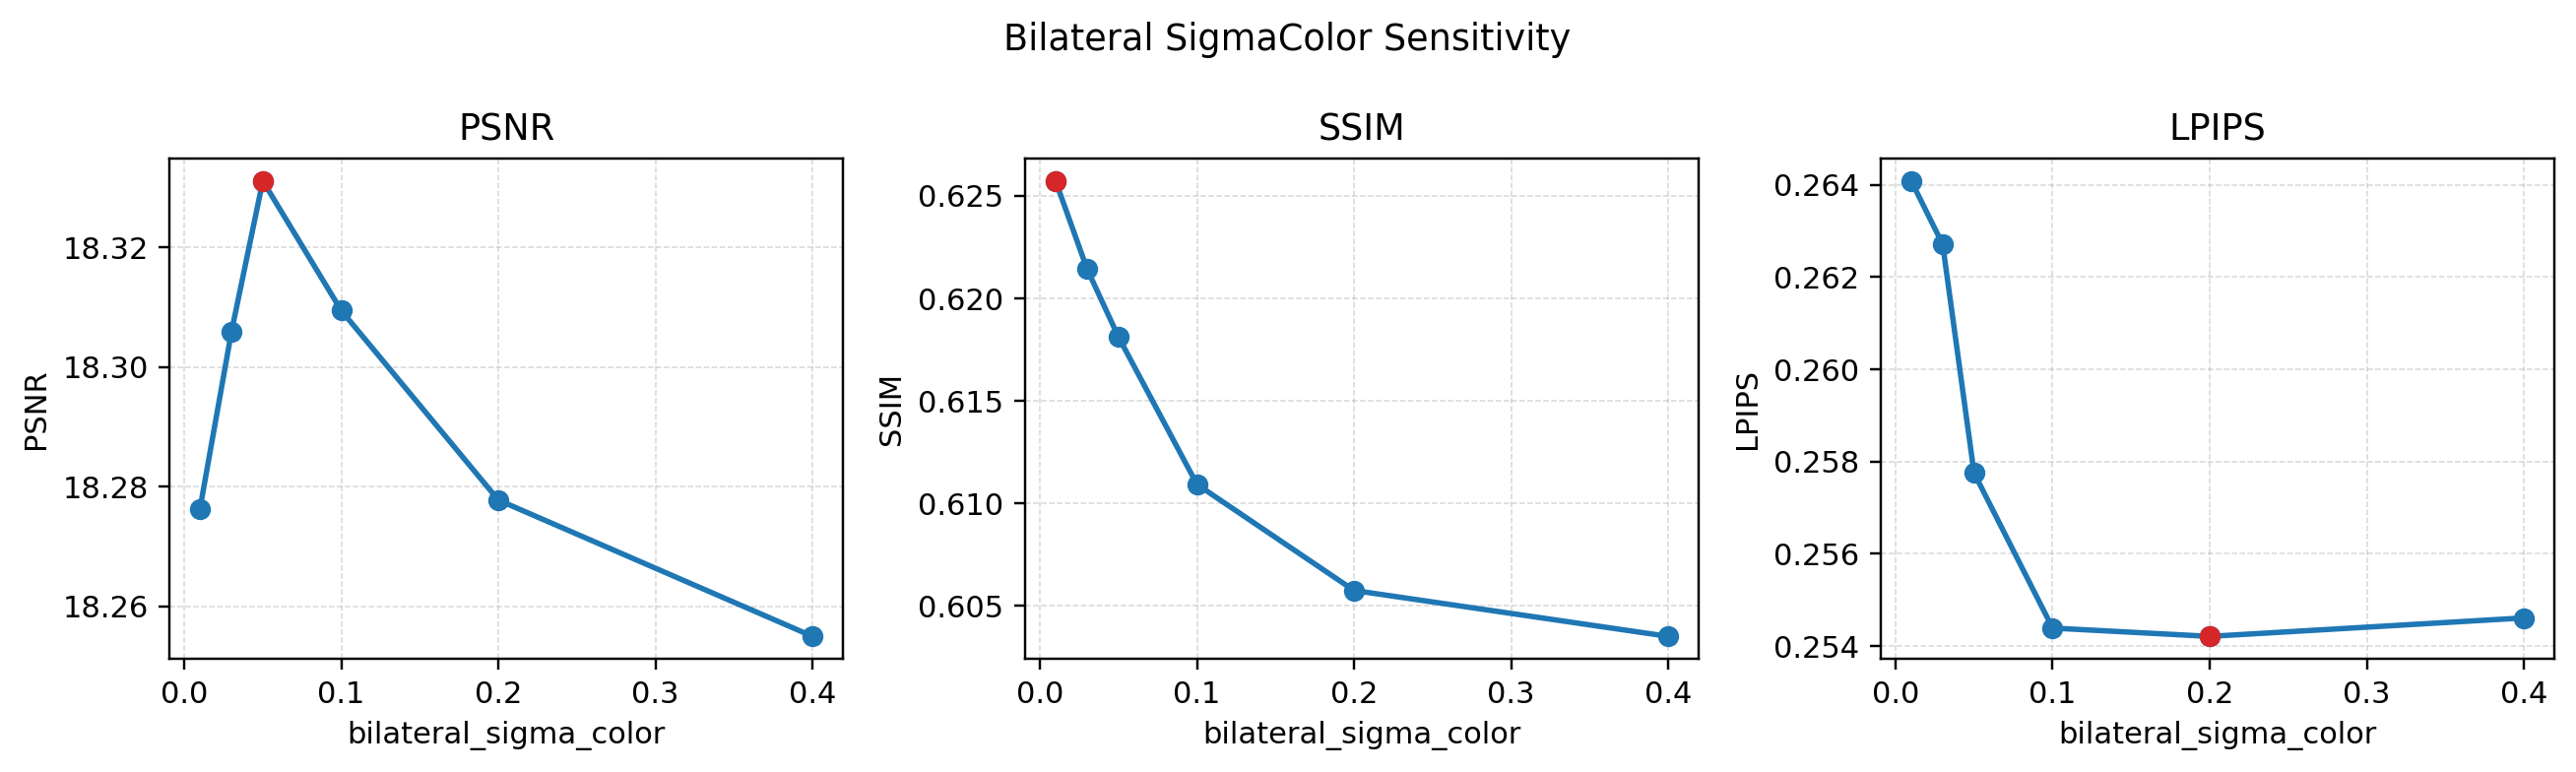
\includegraphics[width=\linewidth]{../assets/figures/bilateral_sigma_color_curve.png}
    \caption{双边滤波值域参数变化对平均指标的影响。}
    \label{fig:bilateral_sigma_color_curve}
\end{figure}

\paragraph{双边滤波空间域参数 $\sigma_{space}$}
表 \ref{tab:bilateral_sigma_space} 与图 \ref{fig:bilateral_sigma_space_curve} 给出了 $\sigma_{space}=3,7,15,30,60,90$ 时的结果。与前两个参数相比，$\sigma_{space}$ 对五项平均指标的影响明显更弱，各组结果几乎保持稳定，仅在较小的 $\sigma_{space}$ 下 SSIM 略高。这表明在当前默认直径 $d=15$ 的设定下，空间域高斯衰减在有效邻域内已经较为稳定，继续增大 $\sigma_{space}$ 并不会显著改变权重分布。

\begin{table}[t]
    \centering
    \caption{双边滤波空间域参数 $\sigma_{space}$ 的影响}
    \label{tab:bilateral_sigma_space}
    \begin{tabular}{cccc}
        \toprule
        $\sigma_{space}$ & PSNR$\uparrow$ & SSIM$\uparrow$ & LPIPS$\downarrow$ \\
        \midrule
        3  & \textbf{18.3106} & \textbf{0.6127} & 0.2576 \\
        7  & \textbf{18.3107} & 0.6113 & 0.2547 \\
        15 & 18.3094 & 0.6109 & 0.2544 \\
        30 & 18.3091 & 0.6108 & 0.2543 \\
        60 & 18.3090 & 0.6108 & 0.2543 \\
        90 & 18.3090 & 0.6108 & \textbf{0.2543} \\
        \bottomrule
    \end{tabular}
\end{table}

\begin{figure}[t]
    \centering
    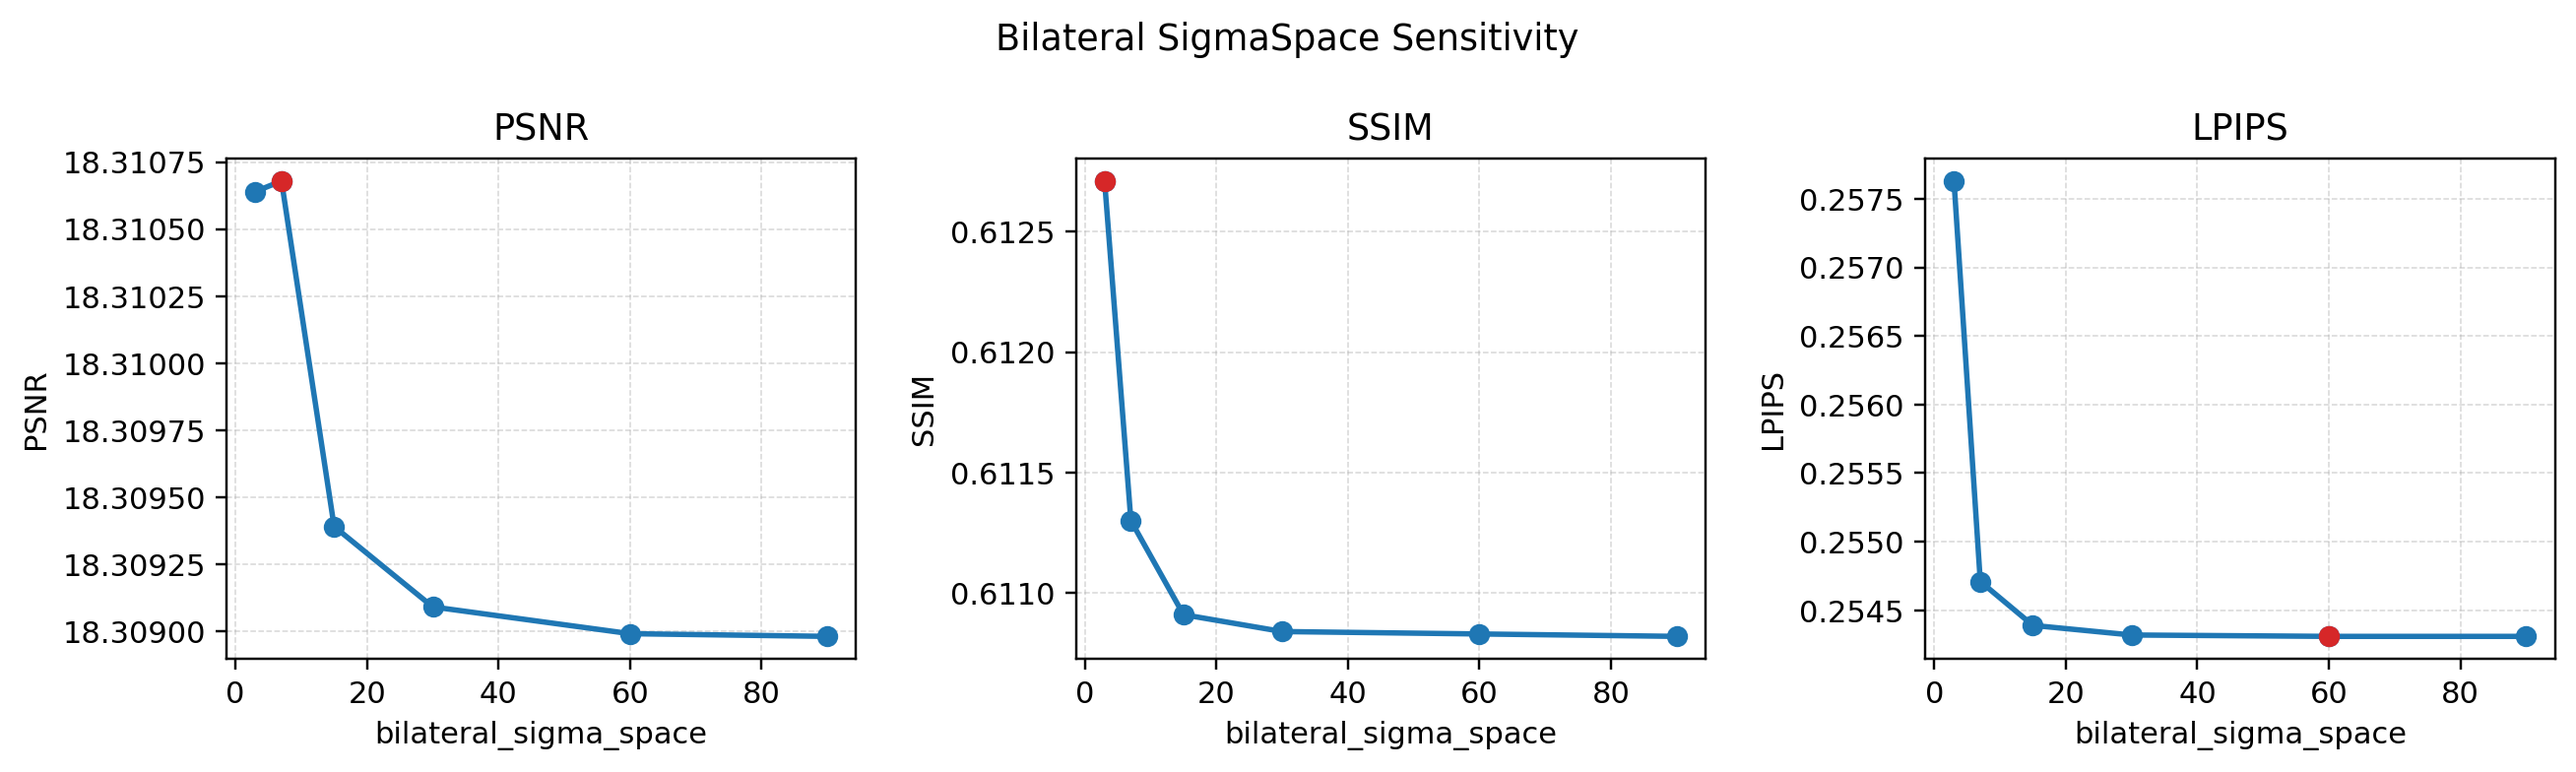
\includegraphics[width=\linewidth]{../assets/figures/bilateral_sigma_space_curve.png}
    \caption{双边滤波空间域参数变化对平均指标的影响。}
    \label{fig:bilateral_sigma_space_curve}
\end{figure}

\begin{figure}[t]
    \centering
    \subcaptionbox{$d=3$}{
        
\includegraphics[width=0.31\linewidth]{../assets/experiments/bilateral_d3/smooth/00017.png}
    }
    \hfill
    \subcaptionbox{$d=35$}{
        
\includegraphics[width=0.31\linewidth]{../assets/experiments/bilateral_d35/smooth/00017.png}
    }
    \hfill
    \subcaptionbox{$\sigma_{color}=0.01$}{
        
\includegraphics[width=0.31\linewidth]{../assets/experiments/bilateral_sc001/smooth/00017.png}
    }
    \\
    \subcaptionbox{$\sigma_{color}=0.40$}{
        
\includegraphics[width=0.31\linewidth]{../assets/experiments/bilateral_sc040/smooth/00017.png}
    }
    \hfill
    \subcaptionbox{$\sigma_{space}=3$}{
        
\includegraphics[width=0.31\linewidth]{../assets/experiments/bilateral_ss3/smooth/00017.png}
    }
    \hfill
    \subcaptionbox{$\sigma_{space}=90$}{
        
\includegraphics[width=0.31\linewidth]{../assets/experiments/bilateral_ss90/smooth/00017.png}
    }
    \caption{样本 \texttt{00017.png} 在双边滤波不同参数下的照明图平滑结果。可以看到，$d$ 和 $\sigma_{color}$ 对局部结构影响更明显，而 $\sigma_{space}$ 的变化相对较弱。}
    \label{fig:bilateral_qualitative}
\end{figure}

综合上述三组实验可以看出，双边滤波在当前任务中对邻域直径 $d$ 最敏感，其次是值域参数 $\sigma_{color}$，而空间域参数 $\sigma_{space}$ 的影响最小。若目标是提升像素级保真与整体感知质量，则较大的 $d$ 和中等偏小的 $\sigma_{color}$ 更有利；若强调结构保持，则应避免将 $\sigma_{color}$ 取值过大。

\paragraph{引导滤波半径 $r$}
表 \ref{tab:guided_radius} 与图 \ref{fig:guided_radius_curve} 给出了 6 组窗口半径实验结果。可以看到，在 $r=2$ 到 $r=32$ 的测试范围内，PSNR 与 SSIM 持续上升，MAE、MSE 与 LPIPS 持续下降，说明更大的局部窗口有助于在更大尺度上估计照明趋势，减少初始照明图中的纹理残留。以 $r=2$ 与 $r=32$ 对比为例，PSNR 从 18.3217 dB 提升到 18.6570 dB，SSIM 从 0.6192 提升到 0.6368，LPIPS 从 0.2631 降低到 0.2386，表明 guided filter 在当前数据范围内尚未出现因窗口过大而导致的明显过平滑。

\begin{table}[t]
    \centering
    \caption{引导滤波半径 $r$ 的影响}
    \label{tab:guided_radius}
    \begin{tabular}{cccccc}
        \toprule
        $r$ & PSNR$\uparrow$ & SSIM$\uparrow$ & MAE$\downarrow$ & MSE$\downarrow$ & LPIPS$\downarrow$ \\
        \midrule
        2  & 18.3217 & 0.6192 & 0.1144 & 0.0199 & 0.2631 \\
        4  & 18.3751 & 0.6229 & 0.1136 & 0.0196 & 0.2546 \\
        8  & 18.4591 & 0.6285 & 0.1122 & 0.0193 & 0.2486 \\
        16 & 18.5615 & 0.6338 & 0.1105 & 0.0188 & 0.2432 \\
        24 & 18.6199 & 0.6357 & 0.1095 & 0.0185 & 0.2402 \\
        32 & \textbf{18.6570} & \textbf{0.6368} & \textbf{0.1088} & \textbf{0.0183} & \textbf{0.2386} \\
        \bottomrule
    \end{tabular}
\end{table}

\begin{figure}[t]
    \centering
    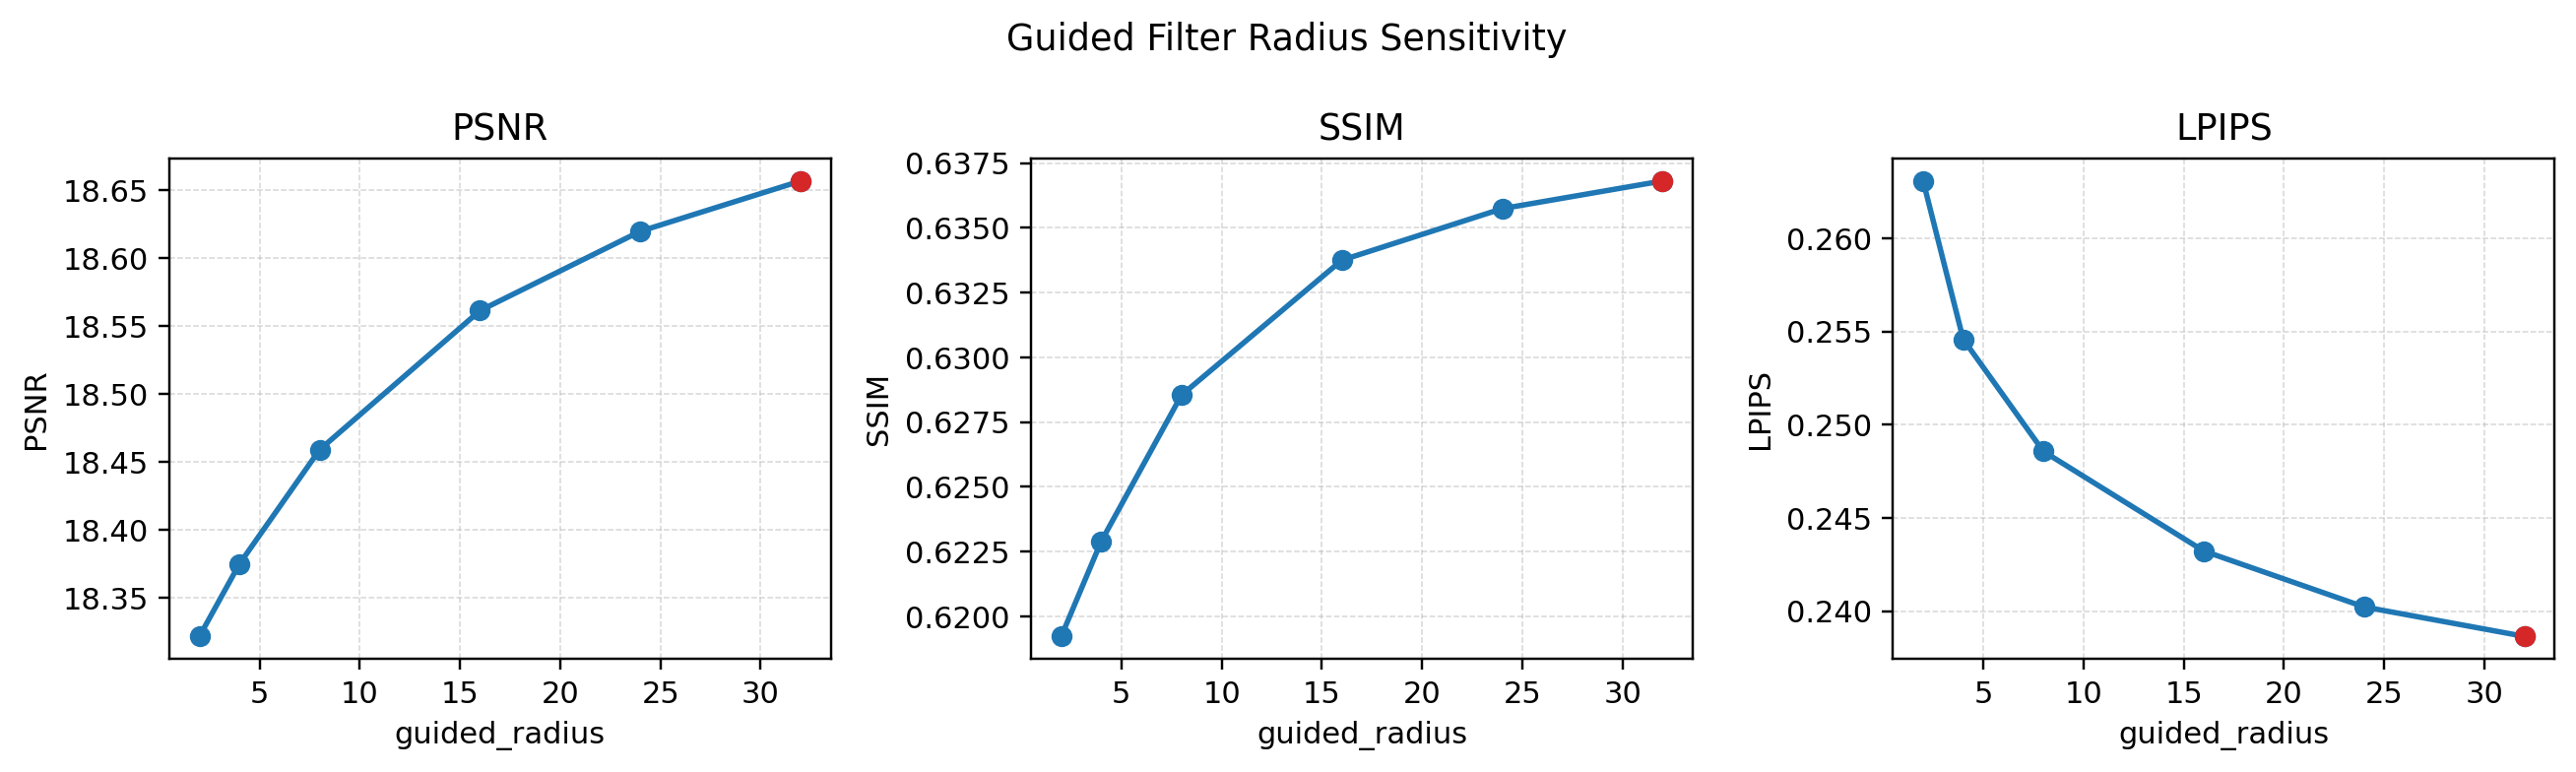
\includegraphics[width=\linewidth]{../assets/figures/guided_radius_curve.png}
    \caption{引导滤波半径变化对平均指标的影响。}
    \label{fig:guided_radius_curve}
\end{figure}

\paragraph{引导滤波正则参数 $\epsilon$}
正则参数 $\epsilon$ 控制局部线性模型对方差项的抑制强度。表 \ref{tab:guided_eps} 与图 \ref{fig:guided_eps_curve} 显示，$\epsilon$ 对结果的影响呈现明显的折中关系。$\epsilon$ 过小时，局部模型过于贴近原始 $T_0$，导致纹理和噪声残留较多；$\epsilon$ 过大时，局部线性系数被过度约束，结构边界会被额外平滑，进而使 SSIM 明显下降。在当前实验中，$\epsilon=10^{-3}$ 取得最高 PSNR 和最低 LPIPS，而 $\epsilon=10^{-4}$ 的 SSIM 略高，说明像素保真、结构一致性和感知质量的最优点并不完全重合。进一步增大到 $\epsilon=10^{-2}$ 与 $10^{-1}$ 后，虽然 MAE/MSE 仍保持较低水平，但 SSIM 从 0.6285 降至 0.6138 和 0.6067，说明过强的正则化会削弱局部结构恢复能力。

\begin{table}[t]
    \centering
    \caption{引导滤波正则参数 $\epsilon$ 的影响}
    \label{tab:guided_eps}
    \begin{tabular}{cccccc}
        \toprule
        $\epsilon$ & PSNR$\uparrow$ & SSIM$\uparrow$ & MAE$\downarrow$ & MSE$\downarrow$ & LPIPS$\downarrow$ \\
        \midrule
        $10^{-6}$ & 18.2727 & 0.6280 & 0.1156 & 0.0202 & 0.2663 \\
        $10^{-5}$ & 18.2822 & 0.6299 & 0.1155 & 0.0202 & 0.2612 \\
        $10^{-4}$ & 18.3318 & \textbf{0.6317} & 0.1147 & 0.0200 & 0.2542 \\
        $10^{-3}$ & \textbf{18.4591} & 0.6285 & 0.1122 & 0.0193 & \textbf{0.2486} \\
        $10^{-2}$ & 18.3970 & 0.6138 & \textbf{0.1112} & \textbf{0.0190} & 0.2499 \\
        $10^{-1}$ & 18.3121 & 0.6067 & 0.1114 & 0.0191 & 0.2521 \\
        \bottomrule
    \end{tabular}
\end{table}

\begin{figure}[t]
    \centering
    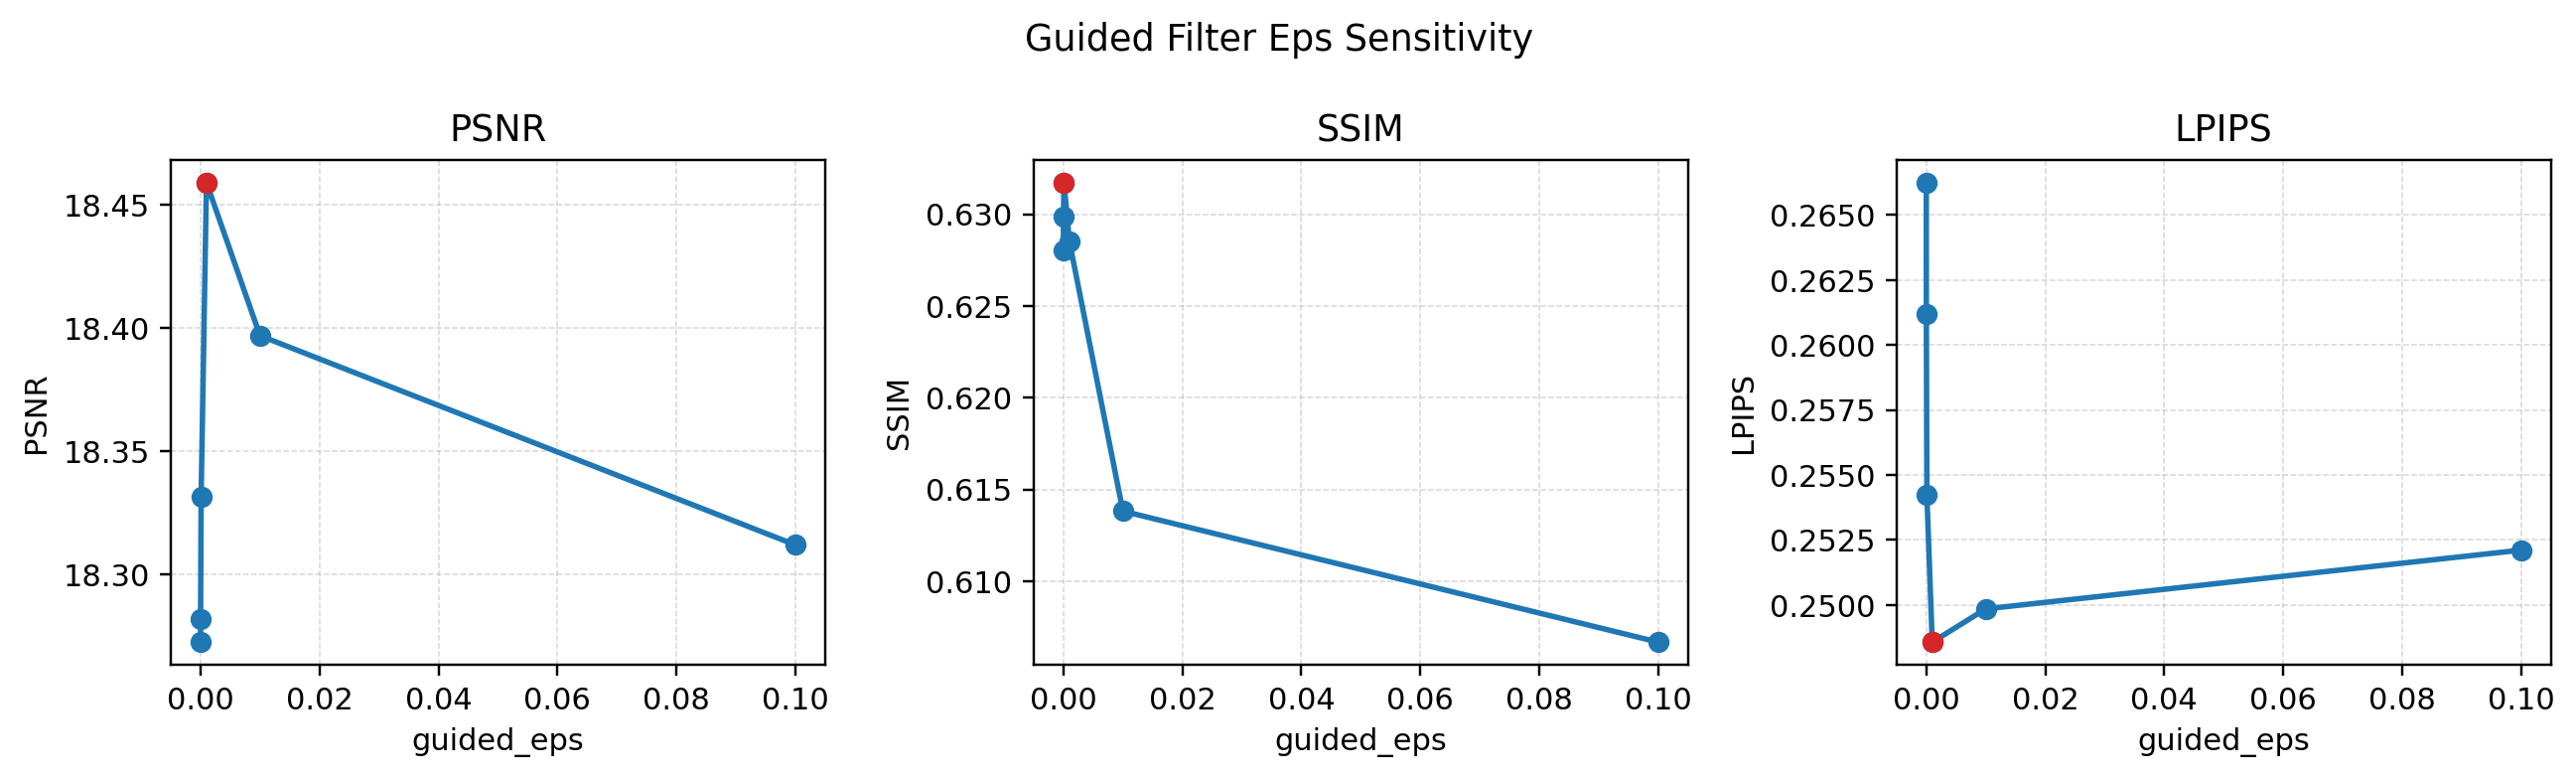
\includegraphics[width=\linewidth]{../assets/figures/guided_eps_curve.png}
    \caption{引导滤波正则参数变化对平均指标的影响。}
    \label{fig:guided_eps_curve}
\end{figure}

\begin{figure}[t]
    \centering
    \subcaptionbox{$r=2$ 时的平滑照明图}{
        
\includegraphics[width=0.48\linewidth]{../assets/experiments/guided_r2/smooth/00017.png}
    }
    \hfill
    \subcaptionbox{$r=32$ 时的平滑照明图}{
        
\includegraphics[width=0.48\linewidth]{../assets/experiments/guided_r32/smooth/00017.png}
    }\\[0.5em]
    \subcaptionbox{$\epsilon=10^{-6}$ 时的平滑照明图}{
        
\includegraphics[width=0.48\linewidth]{../assets/experiments/guided_eps1e-6/smooth/00017.png}
    }
    \hfill
    \subcaptionbox{$\epsilon=10^{-1}$ 时的平滑照明图}{
        
\includegraphics[width=0.48\linewidth]{../assets/experiments/guided_eps1e-1/smooth/00017.png}
    }
    \caption{样本 \texttt{00017.png} 在不同引导滤波参数下的平滑照明图对比。增大半径会使照明估计更趋于全局一致；过大的 $\epsilon$ 会减弱局部结构响应，使边界区域出现更明显的平滑。}
    \label{fig:guided_intermediate}
\end{figure}

\paragraph{增强下限参数 $T_{\min}$}
$T_{\min}$ 用于限制分母中的最小照明值，从而避免极暗区域被过度放大。表 \ref{tab:tmin} 与图 \ref{fig:tmin_curve} 显示，$T_{\min}$ 的变化同样会显著影响增强结果，但其影响方式与 $\gamma$ 不同。较小的 $T_{\min}$ 会允许更强的暗区补偿，因此在像素误差指标上可能更有优势，例如 $T_{\min}=0.05$ 时取得最高 PSNR 18.8776 dB 和最低 MSE 0.0153；但此时暗区噪声也更容易被放大，导致 LPIPS 仍处于较高水平。随着 $T_{\min}$ 增大到 0.10 和 0.15，补偿强度逐渐受限，图像整体更加稳定，结构相似性和感知质量更好，其中 $T_{\min}=0.15$ 取得最高 SSIM 0.6291 和最低 LPIPS 0.2362。若继续增大到 0.25，则会明显压制暗区恢复，整体图像偏暗，PSNR 与 SSIM 同时下降。综合来看，$T_{\min}$ 控制的是“是否允许极暗区域被大幅拉升”，因此它在保真、结构和感知指标之间体现出明显的多目标折中。

\begin{table}[t]
    \centering
    \caption{增强下限参数 $T_{\min}$ 的影响（基于引导滤波）}
    \label{tab:tmin}
    \begin{tabular}{cccccc}
        \toprule
        $T_{\min}$ & PSNR$\uparrow$ & SSIM$\uparrow$ & MAE$\downarrow$ & MSE$\downarrow$ & LPIPS$\downarrow$ \\
        \midrule
        0.02 & 18.3716 & 0.5912 & 0.1001 & 0.0166 & 0.3086 \\
        0.05 & \textbf{18.8776} & 0.6067 & \textbf{0.0974} & \textbf{0.0153} & 0.2845 \\
        0.08 & 18.8741 & 0.6219 & 0.1023 & 0.0166 & 0.2616 \\
        0.10 & 18.4591 & 0.6285 & 0.1122 & 0.0193 & 0.2486 \\
        0.15 & 15.7750 & \textbf{0.6291} & 0.1648 & 0.0348 & \textbf{0.2362} \\
        0.25 & 11.3799 & 0.5631 & 0.2678 & 0.0819 & 0.2490 \\
        \bottomrule
    \end{tabular}
\end{table}

\begin{figure}[t]
    \centering
    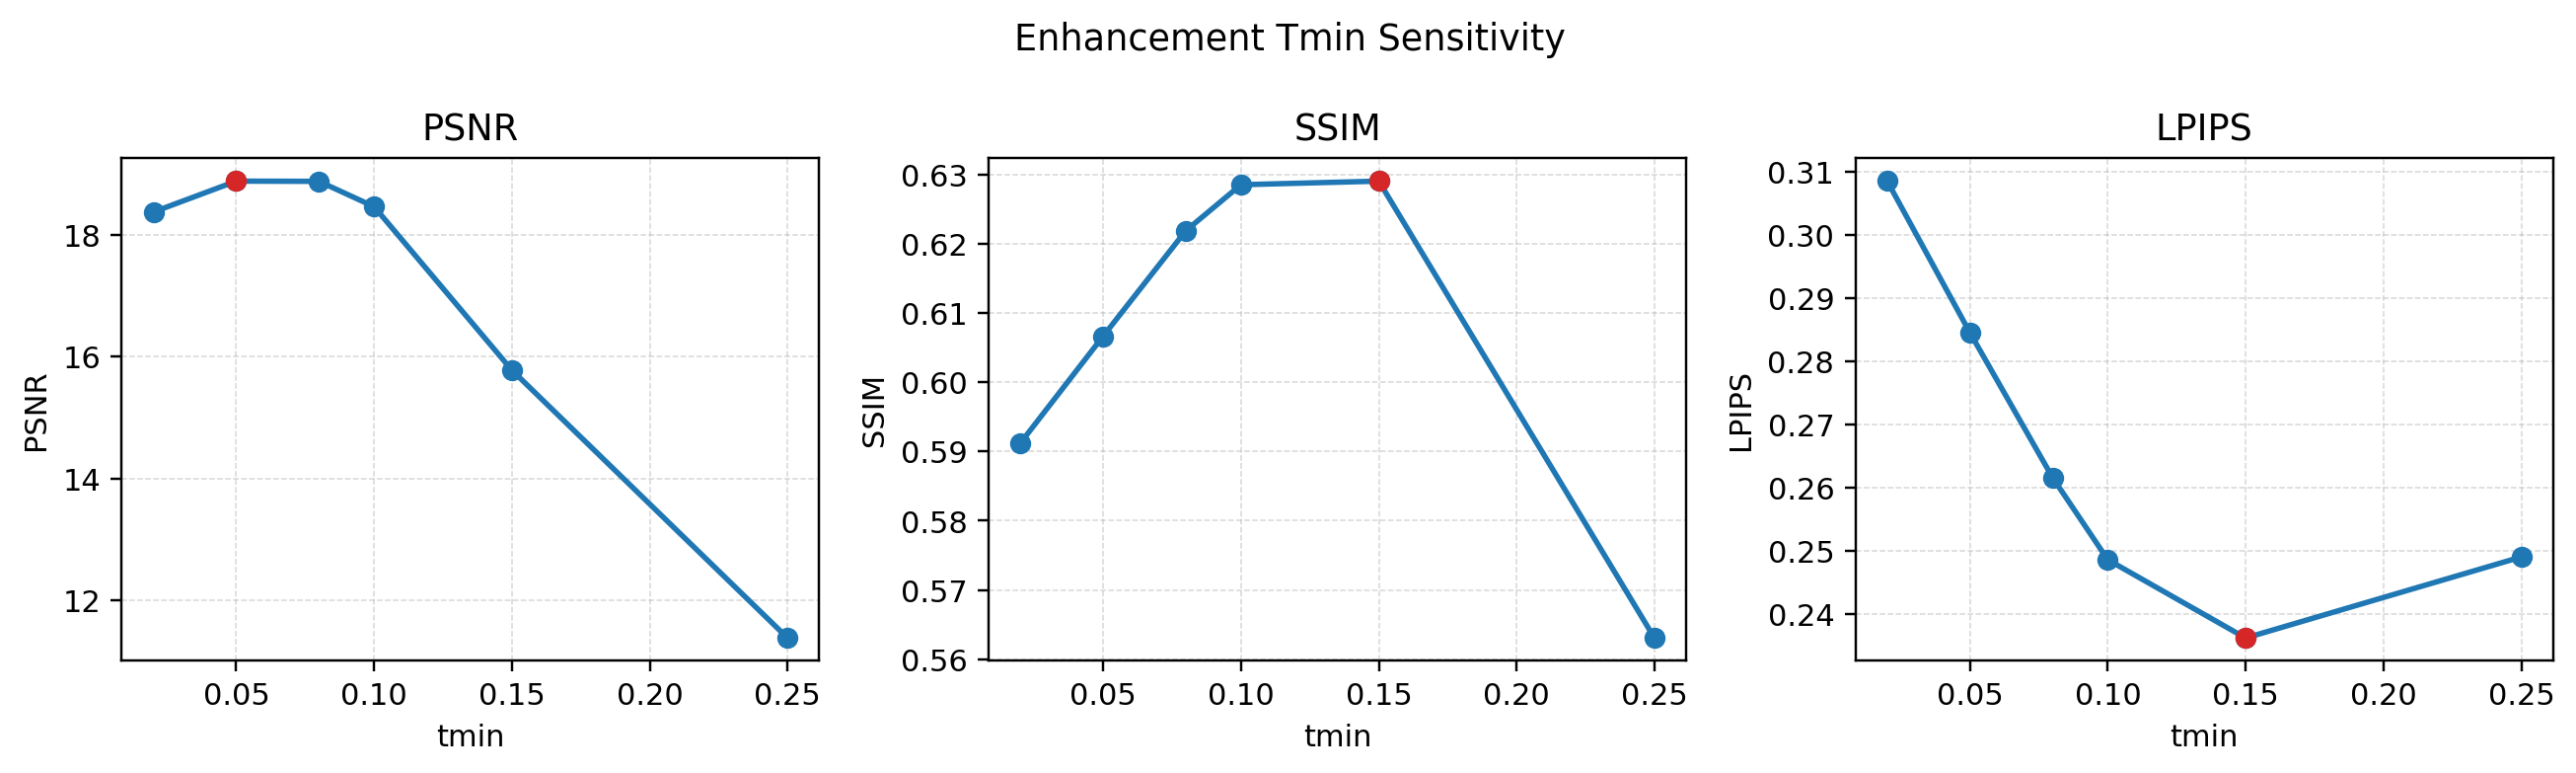
\includegraphics[width=\linewidth]{../assets/figures/guided_tmin_curve.png}
    \caption{增强下限参数 $T_{\min}$ 变化对平均指标的影响。}
    \label{fig:tmin_curve}
\end{figure}

\begin{figure}[t]
    \centering
    \subcaptionbox{$T_{\min}=0.02$}{
        
\includegraphics[width=0.31\linewidth]{../assets/experiments/guided_tmin002/enhanced/00017.png}
    }
    \hfill
    \subcaptionbox{$T_{\min}=0.05$}{
        
\includegraphics[width=0.31\linewidth]{../assets/experiments/guided_tmin005/enhanced/00017.png}
    }
    \hfill
    \subcaptionbox{$T_{\min}=0.08$}{
        
\includegraphics[width=0.31\linewidth]{../assets/experiments/guided_tmin008/enhanced/00017.png}
    }
    \\
    \subcaptionbox{$T_{\min}=0.10$}{
        
\includegraphics[width=0.31\linewidth]{../assets/experiments/guided_tmin010/enhanced/00017.png}
    }
    \hfill
    \subcaptionbox{$T_{\min}=0.15$}{
        
\includegraphics[width=0.31\linewidth]{../assets/experiments/guided_tmin015/enhanced/00017.png}
    }
    \hfill
    \subcaptionbox{$T_{\min}=0.25$}{
        
\includegraphics[width=0.31\linewidth]{../assets/experiments/guided_tmin025/enhanced/00017.png}
    }
    \caption{样本 \texttt{00017.png} 在不同增强下限参数下的增强结果。较小的 $T_{\min}$ 会更强烈地拉升暗区，同时更容易放大噪声；较大的 $T_{\min}$ 则会抑制过增强，但也可能使整体亮度恢复不足。}
    \label{fig:tmin_qualitative}
\end{figure}

\paragraph{增强指数 $\gamma$}
增强公式中的 $\gamma$ 直接控制照明补偿强度，因此其影响最为直观。表 \ref{tab:gamma} 与图 \ref{fig:gamma_curve} 显示，在本实验选取的 6 组参数中，$\gamma=0.8$ 的综合表现最好，其 PSNR、SSIM 分别达到 18.4591 dB 和 0.6285，同时保持较低的 MSE 与较好的 LPIPS。与之相比，较小的 $\gamma=0.4$ 和 $\gamma=0.6$ 会导致增强不足，大面积暗区无法被充分拉升，因此像素误差较大；而当 $\gamma$ 增大到 1.0 以上时，亮度补偿过强，噪声和局部失真被同步放大，SSIM、PSNR 与 LPIPS 均显著恶化。例如，当 $\gamma$ 从 0.8 增加到 1.4 时，PSNR 从 18.4591 dB 下降到 8.7632 dB，LPIPS 从 0.2486 恶化到 0.5777，说明过增强对定量质量破坏非常明显。

\begin{table}[t]
    \centering
    \caption{增强指数 $\gamma$ 的影响（基于引导滤波）}
    \label{tab:gamma}
    \begin{tabular}{cccccc}
        \toprule
        $\gamma$ & PSNR$\uparrow$ & SSIM$\uparrow$ & MAE$\downarrow$ & MSE$\downarrow$ & LPIPS$\downarrow$ \\
        \midrule
        0.4 & 9.2020  & 0.4763 & 0.3342 & 0.1283 & 0.2688 \\
        0.6 & 12.2243 & 0.6090 & 0.2403 & 0.0675 & \textbf{0.2430} \\
        0.8 & \textbf{18.4591} & \textbf{0.6285} & \textbf{0.1122} & \textbf{0.0193} & 0.2486 \\
        1.0 & 14.3550 & 0.5360 & 0.1671 & 0.0410 & 0.3148 \\
        1.2 & 10.6393 & 0.5185 & 0.2632 & 0.0951 & 0.4570 \\
        1.4 & 8.7632  & 0.4750 & 0.3256 & 0.1396 & 0.5777 \\
        \bottomrule
    \end{tabular}
\end{table}

\begin{figure}[t]
    \centering
    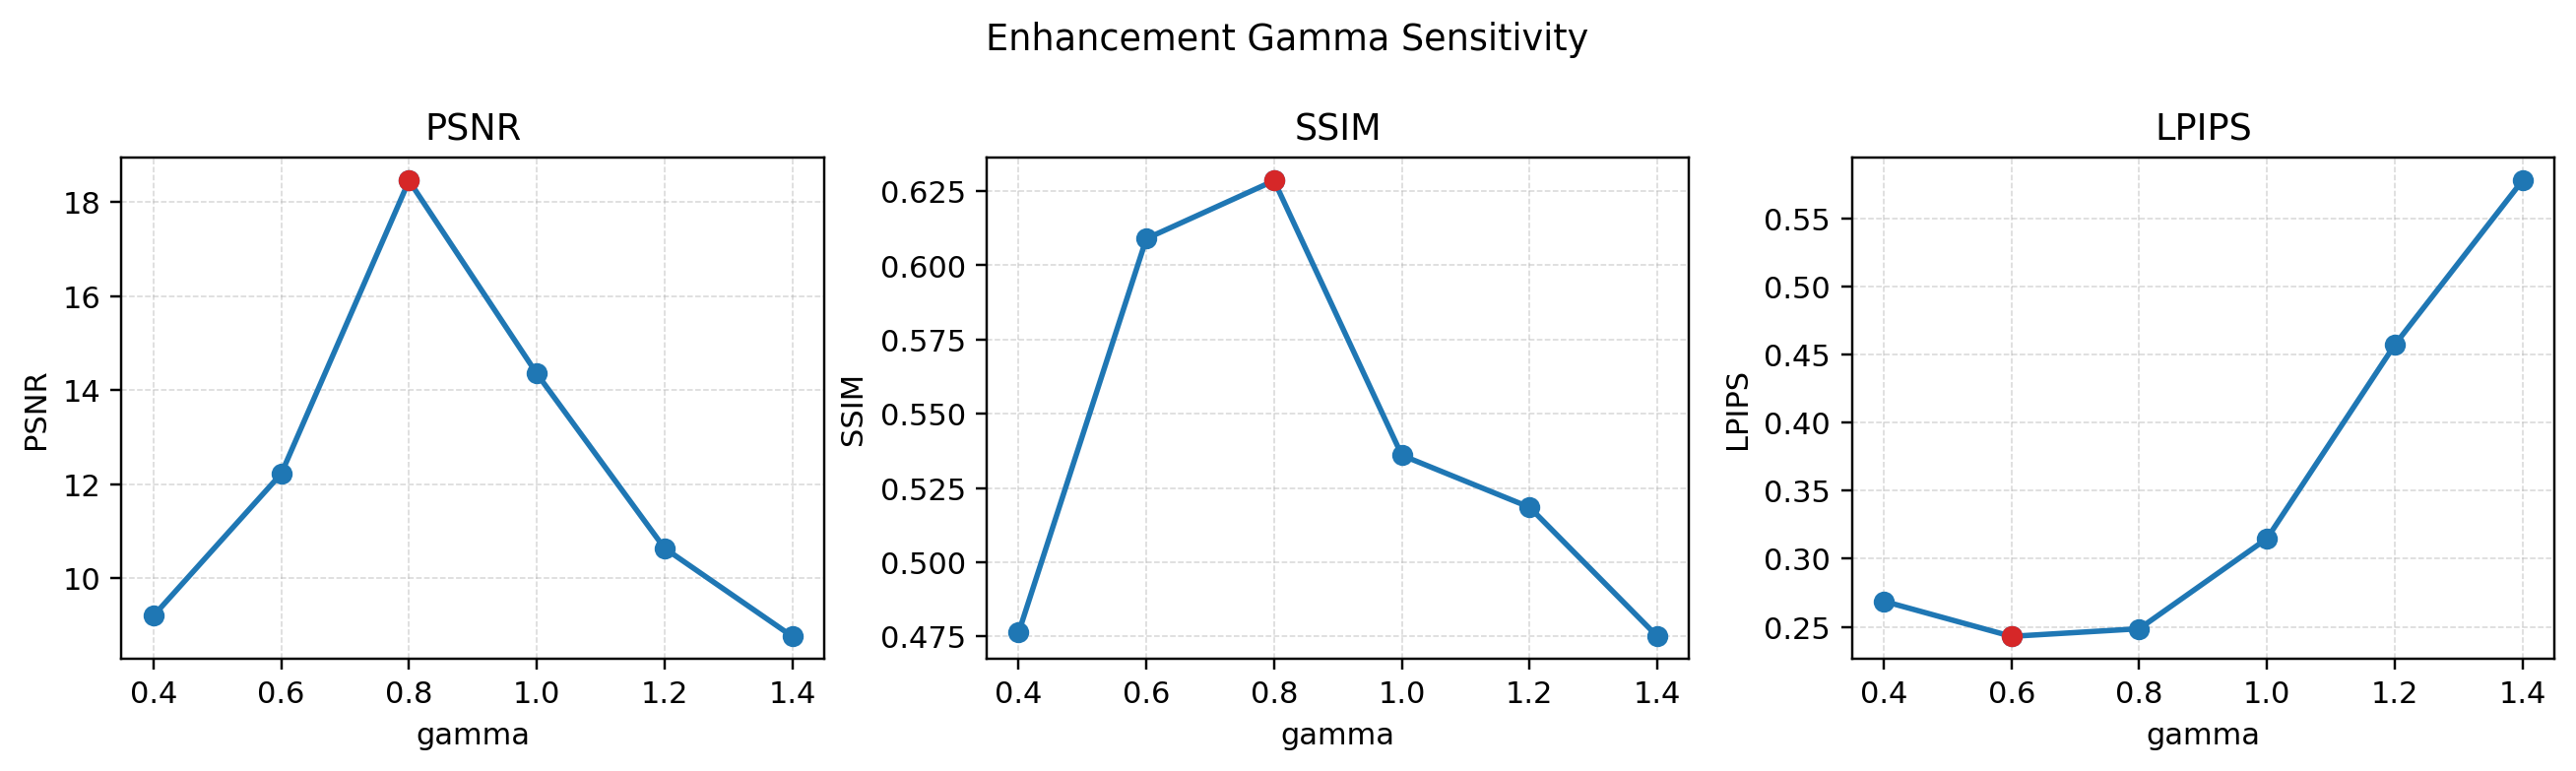
\includegraphics[width=\linewidth]{../assets/figures/guided_gamma_curve.png}
    \caption{增强指数 $\gamma$ 变化对平均指标的影响。}
    \label{fig:gamma_curve}
\end{figure}

\begin{figure}[t]
    \centering
    \subcaptionbox{$\gamma=0.4$}{
        
\includegraphics[width=0.31\linewidth]{../assets/experiments/guided_gamma04/enhanced/00017.png}
    }
    \hfill
    \subcaptionbox{$\gamma=0.6$}{
        
\includegraphics[width=0.31\linewidth]{../assets/experiments/guided_gamma06/enhanced/00017.png}
    }
    \hfill
    \subcaptionbox{$\gamma=0.8$}{
        
\includegraphics[width=0.31\linewidth]{../assets/experiments/guided_gamma08/enhanced/00017.png}
    }
    \\
    \subcaptionbox{$\gamma=1.0$}{
        
\includegraphics[width=0.31\linewidth]{../assets/experiments/guided_gamma10/enhanced/00017.png}
    }
    \hfill
    \subcaptionbox{$\gamma=1.2$}{
        
\includegraphics[width=0.31\linewidth]{../assets/experiments/guided_gamma12/enhanced/00017.png}
    }
    \hfill
    \subcaptionbox{$\gamma=1.4$}{
        
\includegraphics[width=0.31\linewidth]{../assets/experiments/guided_gamma14/enhanced/00017.png}
    }
    \caption{样本 \texttt{00017.png} 在不同增强指数下的增强结果。较小的 $\gamma$ 会导致整体偏暗、增强不足；较大的 $\gamma$ 虽能显著提亮暗区，但会同时带来更强的噪声放大和局部过曝。}
    \label{fig:gamma_qualitative}
\end{figure}

\section{总结}
本文完成了一个基于 Retinex 思想的低光照图像增强实验系统，重点比较了双边滤波与引导滤波两种照明图平滑方式，并通过定量与定性实验分析了关键参数对结果的影响。实验表明：
\begin{enumerate}
    \item 在默认参数下，引导滤波优于双边滤波，说明局部线性约束更适合本作业数据中的照明图细化；
    \item 对双边滤波而言，邻域直径 $d$ 的影响最显著，值域参数 $\sigma_{color}$ 次之，而空间域参数 $\sigma_{space}$ 的影响最弱；
    \item 对引导滤波而言，较大的窗口半径在当前样本上表现更稳定，而正则参数 $\epsilon$ 则体现出明显的保边与过平滑折中；
    \item 对增强参数而言，$T_{\min}$ 与 $\gamma$ 共同控制暗区补偿幅度，其中较小的 $T_{\min}$ 有利于提升像素级误差指标，但更容易放大噪声；$\gamma=0.8$ 在当前数据上取得了最平衡的结果，过小会增强不足，过大则会导致明显的过增强和感知质量恶化。
\end{enumerate}

本文方法的优点是结构清晰、实现简单、可解释性强，并且能够直接输出初始照明图、平滑照明图和增强结果等中间步骤。其不足在于：第一，照明估计仍采用最大通道近似，难以应对复杂光照和严重色偏；第二，参数仍依赖人工设置，不同图像上的最优取值并不完全一致；第三，在极暗样本中，增强后仍会放大噪声，与 GT 之间存在亮度偏差。后续可尝试更稳健的照明图先验、联合去噪机制，或引入学习型方法进一步提升结果。

{\small
\bibliographystyle{ieeenat_fullname}
\bibliography{references}
}

\end{document}
